\documentclass[10pt,conference]{IEEEtran}

\usepackage{balance}
\usepackage[pdftex]{graphicx} % St�tte for bilder inkl. pdf
\usepackage{amsmath}
\usepackage{algorithm}
\usepackage{algpseudocode}
\usepackage{todonotes}
\usepackage{hyperref}

\graphicspath{{./img/}}
\graphicspath{{./gnuplot/}}

\newcommand{\superscript}[1]{\ensuremath{^{\textrm{#1}}}}
\newcommand{\subscript}[1]{\ensuremath{_{\textrm{#1}}}}
\newcommand{\comment}[1]{}

\newcommand{\speedup}{1.104 }

\hypersetup{colorlinks=true, 
			linkcolor=black, 
			filecolor=black,
			citecolor=black,
			urlcolor=black}

\begin{document}

\title{Pattern Matching Prefetcher}

\author{
        Sivert~Berg,~\IEEEmembership{Student,~NTNU,}
        Anders~B.~Eie,~\IEEEmembership{Student,~NTNU,}\\
        Ole~Petter~Skarre~Lund,~\IEEEmembership{Student,~NTNU}
        and~Simen~Natvig~\IEEEmembership{Student,~NTNU}}

\maketitle

\begin{abstract}
In this paper we present a stride prefetcher that uses pattern matching and
most common stride. It is influenced by Delta Correlation Prediction Table
prefetchers, but instead of storing delta values it stores addresses.

The prefetcher first looks for a perfect or partial matching among the delta
values calculated from the addresses, but if that fails it looks for the most
common stride.

Using the SPEC CPU2000 benchmark suite together with the M5 simulator, the
resulting prefetcher achieves an average speedup of 10.4\% compared to no
prefetcher at all. Max achieved speedup was 60.5\% with the \emph{ammp} program.

\end{abstract}

\section{Introduction}
The gap between processor speed and main memory speed has for many years increased dramatically. To
attack this problem several solutions has been proposed and implemented. One of them is prefetching
where the processor gets the instruction and data before it is used so it doesn't have to wait for
it when it actually has to use it. Prefetching helps to decrease the average memory access time
and thereby increases the overall computer efficiency.

Several schemes can be used to implement a prefetcher. Our prefetcher uses a scheme called
\emph{stride}. It essentially consists of a table that is index by the program counter (PC) and it
stores, amongst other things, a stride that is the difference between the two most recent miss
addresses for a particular program counter address. When the prefetcher detects a pattern in the
strides it uses the stride value to prefetch what it assumes to be data that the processor needs in
the near future.



\section{Related Work}
A lot of work has been done in this field, resulting in many different prefetching heuristics. They
range from the very simple sequential ones, that simply fetches the address after the current one,
to more complex ones that tries to find patterns and use dynamically gathered statistics to guide
them \cite{prefetch_range}.

\subsection{Reference Prediction Tables}
Reference Prediction Tables (RPT) \cite{rpt} is a prefetching technique which uses a large table to
store information indexed by the program counter of the load. It calculates the delta for each miss,
but the prefetching is only done after a certain amount of misses with the delta has occured.

\subsection{Program Counter/Delta Correlation Prefetching}
Program Counter/Delta Correlation Prefetching (PC/DC) \cite{prefetch_range} is a prefetching method
using a Global History Buffer (GHB). It uses buffered delta calculations to search for stride
patterns. If a pattern is found, it is used to start prefetching.

\subsection{Delta Correlation Prediction Tables} 
Delta Correlation Prediction Tables combines RPT and PC/DC \cite{dcpt}. A large table is indexed by the program counter and Fig.~\ref{fig:dcpt_entry} shows an
entry in the table.
\begin{figure}[h]
	\begin{center}
		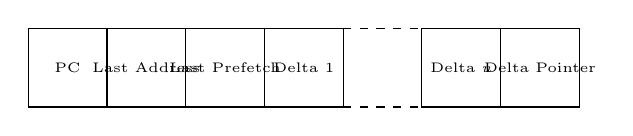
\begin{tikzpicture}
			\draw (0,0) rectangle (1,1);
			\draw (1,0) rectangle (2,1);
			\draw (2,0) rectangle (3,1);
			\draw (3,0) rectangle (4,1);
			\draw[dashed] (4,0) -- (5,0);
			\draw[dashed] (4,1) -- (5,1);
			\draw (5,0) rectangle (6,1);
			\draw (6,0) rectangle (7,1);

			\draw (0.5,0.5) node {\tiny PC};
			\draw (1.5,0.5) node {\tiny Last Address};	
			\draw (2.5,0.5) node {\tiny Last Prefetch};
			\draw (3.5,0.5) node {\tiny Delta 1};
			\draw (5.5,0.5) node {\tiny Delta \emph{n}};
			\draw (6.5,0.5) node {\tiny Delta Pointer};
		\end{tikzpicture}
	\end{center}
	\caption{DCPT entry\label{fig:dcpt_entry}}
\end{figure}
The \emph{PC} field contains the program counter of the load instruction. \emph{Last address}
contains the load address. The \emph{delta} fields contains the calculated delta values for this
load instruction. These delta fields works as a circular buffer, where the \emph{delta pointer}
field points to the head of the buffer. \emph{Last prefetch} stores the last prefetch address. 

When a new delta is calculated, it is stored in the circular buffer and the prefetcher goes through
the buffer to search for a match for the two newest calculated deltas. When a match is found the
first prefetch candidate is calculated by adding the delta after the match to the address in the
\emph{last address} field. The second one is calculated by adding the next delta value to the first
prefetch candidate. This is done for all the delta values after the matched pair, also with the
newest calculated delta values.


\section{Description}
As mentioned above our prefetcher is a stride prefetcher. It tries to detect a 
pattern in the access history, and use this pattern to predict future 
references. Patterns could be detected on a global or a local (per PC) basis.
After reviewing statistics gathered from SPEC CPU2000 benchmarks we decided to 
focus on local patterns. This was because the global access stream had little 
additional unique information that could not already be extracted from the 
local streams without using a lot of additional resources. In most benchmarks 
the memory accesses are done by a few instructions that operate in a very 
predictable fashion. The prefetcher is very similar to a DCPT, but we store just the 
addresses instead of the delta values, and nothing else.

\subsection{Table}

\begin{figure}
	\begin{tikzpicture}
		\draw [->] (1,7.5) -- (2, 7.5);
		\draw (1.5, 7.8) node {PC};
		\foreach \x in {6,...,8}
			\draw (2, \x) rectangle (3, \x + 1);

		\draw [dotted] (2, 5.75) -- (2, 5.25);
		\draw [dotted] (3, 5.75) -- (3, 5.25);
		\draw (2, 5) -- (2, 5.25);
		\draw (2, 6) -- (2, 5.75);
		\draw (3, 5) -- (3, 5.25);
		\draw (3, 6) -- (3, 5.75);
		\draw (2, 4) rectangle  (3, 5);

		\foreach \x in {0,2}
			\draw (\x * 1.5 + 4, 6.75) rectangle  (\x * 1.5 + 5.5, 8.25);

		\draw [dashed] (3, 8) -- (4, 8.25);
		\draw [dashed] (3, 7) -- (4, 6.75);

		\draw [dotted] (5.5, 6.75) rectangle (7, 8.25);
		\draw (5.5, 6.75) -- (5.75, 6.75);
		\draw (6.75, 6.75) -- (7, 6.75);
		\draw (5.5, 8.25) -- (5.75, 8.25);
		\draw (6.75, 8.25) -- (7, 8.25);

		\draw (4.75, 7.5) node {$a_0$};
		\draw (7.75, 7.5) node {$a_{2n}$};
	\end{tikzpicture}
	\caption{Access History Table}
	\label{fig:table}
\end{figure}

To keep track of the previous memory accesses of a program counter we use a
table. Each table entry contains a list of the last memory accesses and misses
by the program counter that maps to this entry. On a hit or a miss the address
of the access is added at the front of the list corresponding to the program
counter of the instruction that made the access while the rest if shifted on
place to the right. In hardware this would be implemented with a ring buffer. A
graphical representation of the table can be seen in Fig.~\ref{fig:table}. The
exact number of accesses to store in each entry can be tweaked. More addresses
per entry allows larger patterns to be detected, but reduces the number of
entries using the same amount of memory. Larger patterns might allow you to
catch more, while more entries reduces the chance of collision.

To save space we store only the lower $k$ bits in every address. Because the
simulated computer uses 64 byte cache lines, the lower 6 bits of addresses in
the cache will always be 0, and can safely be ignored. With $k=16$ we store
only 10 bits and can correctly identify patterns as long as the biggest stride
is less than $2^{16}$.

Because the table size is much smaller
than the number of possible program counters, several instructions could use
the same table entry. If this happened in a real program it could lead to less
than optimal prefetching. With a sufficiently large table the chance of two
instructions clashing would be negligible. In addition the table entry is found
by taking the program counter modulo the table size. This ensures that
instructions that is less than table size apart will map to different table
entries, meaning all instructions in a small loop is likely to map to different
table entries.

\subsection{Pattern Matching}

When the table begins to fill we are able to find patterns in the memory accesses.
To find these patterns we calculate relative and absolute strides.
The relative stride is the difference between two consecutive
addresses. Absolute strides are calculated by choosing a pattern size n,
and then computing the difference between the address at position
$n$ to every address before $n$, and then doing the same for the address
at position $2n$.

That is,
\[
	s_i = \begin{cases}
		a_i - a_n,    & \text{if } i  < n \\%\in \{0 \dots n -1\}\\
		a_i - a_{2n}, & \text{if } i \geq n % \{n \dots 2n - 1\}
	\end{cases}
\]
where $s_i$~is the $i$th absolute stride, and $a_i$~is the address at position
$i$ in the table. Note that the newest address is at index 0 in the table. A
perfect match is found if
\begin{equation}
\label{eq:match}
\forall i \in \{0 \dots n - 1\} \,.\, s_i = s_{i + n}
\end{equation}

It is also possible to find a partial match. We then simply relax the
requirement in equation \eqref{eq:match} that all strides have to match, to
that at least some percentage has to match.

An example of a perfect match can be seen in Table~\ref{table:pattern}.

%Partial matching is the reason for using absolute strides instead of the
%more intuitive relative stride. If we have a partial match, and use relative
%strides, there is no easy way to prefetch a

\begin{table}[htb]
	\caption{Example of pattern with n=4}
	\label{table:pattern}
	\centering
	\begin{tabular}{c|c|c|c|c}
		\bfseries Position &
		\bfseries Address &
		\bfseries Stride &
		\bfseries Stride &
		\bfseries Stride \\
		& &
		\bfseries (Relative) &
		\bfseries (Absolute) &
		\bfseries Index \\
		\hline
		0 & 896   & & \\
		  &	& 64 & 448 & 0 \\
		1 & 832  & & \\
		  & & 64 & 384 & 1 \\
		2 & 768 & & \\
		  & & 128 & 320 & 2 \\
		3 & 640 & & \\
		  & & 192 & 192 & 3 \\
		4 & 448 & & \\
		  &	& 64 & 448 & 4 \\
		5 & 384 & & \\
		  &	& 64 & 384 & 5 \\
		6 & 320 & & \\
		  &	& 128 & 320 & 6 \\
		7 & 192 & & \\
		  &	& 192 & 192 & 7 \\
		8 & 0 & & \\
	\end{tabular}
\end{table}

\subsection{Most Common Stride}

In addition to the pattern matching above, we also implemented most common stride
prefetching. This was added as a fallback measure if the pattern matching code
was unable to find a pattern.
It looks for the most common relative stride, and if the number
of this stride is over a threshold
it will use it to prefetch a
set number of cache lines.
In Table~\ref{table:pattern} the most common stride is 64.

\subsection{Algorithm}

Pseudocode for the algorithm used can be found in Algorithm~\ref{alg:stride}.
The algorithm first tries to find a pattern of size $n$, then $n-1$ and so
on until it tries to find a pattern of size $1$. If no such patterns are
found it goes on to try finding a most common stride.

As we can see there are a few constants in the algorithm that can be
tuned. These are

~
\begin{itemize}
	\item \textbf{ THRESHOLD\subscript{stride}} \\ Determines when there is a match.
	For perfect matching this should be equal to the pattern size \\
	\item \textbf{ AGGR\subscript{stride}} \\ The aggresiveness determines how many
	cachelines we should prefetch. This is also called prefetch degree \\
	\item \textbf{ THRESHOLD\subscript{mcs}} \\ Sets a lower limit on how many
	there must be of the most commons stride before starting to prefetch \\
	\item \textbf{ AGGR\subscript{mcs}} \\  Same as the stride equivalent \\
\end{itemize}

It is important to note that these ``constants'' are actually C macros in our
source code, so they could depend on any variables in scope on the location
they are used.
Specifically \textbf{THRESHOLD\subscript{stride}} and
\textbf{AGGR\subscript{stride}} could depend on the pattern size.

\algnotext{EndIf}
\algnotext{EndFor}
\algnotext{EndFunction}

\begin{algorithm}
	\caption{The prefetching algorithm}
	\label{alg:stride}
	\begin{algorithmic}
		\Function{prefetch}{$a_0$, $a_1$, \dots, $a_{2n}$}
		\If{$\neg$ \textsc{stride\_prefetch}($a_0$, $a_1$, \dots, $a_{2n}$)}
			\State \textsc{mcs\_prefetch}($a_0$, $a_1$, \dots, $a_{2n}$)
		\EndIf
		\EndFunction
		\\
		\Function{stride\_prefetching}{$a_0$, $a_1$, \dots, $a_{2n}$}
			\For{$i = n \to 1$}
				\State $hits \gets 0$
				\For{$j = 0 \to i - 1$}
					\State $hit_j \gets$ \textnormal{false}
					\State $s_j \gets a_j - a_i$
					\State $s_{i + j} \gets a_{i + j} - a_{2i}$
				\EndFor
				\For{$j = 0 \to i - 1$}
					\If{$s_j \equiv s_{i + j}$}
						\State $hits \gets hits + 1$
						\State $hit_j \gets$ \textnormal{true}
					\EndIf
				\EndFor
				\If{$hits \geq$ THRESHOLD\subscript{stride}}
					\For{$j = 0 \to$ AGGR\subscript{stride}}
						\State $k \gets i - 1 - mod(i,j)$
						\If{$hit_k$}
							\State \textsc{prefetch}($a_0 + s_k + s_0 \cdot (\lfloor \frac{j}{i} \rfloor)$)
						\EndIf
					\EndFor
					\State {\bfseries return} \textnormal{true}
				\EndIf
			\EndFor

			\Return \textnormal{false}
		\EndFunction
		\\
		\Function{mcs\_prefetching}{$a_0$, $a_1$, \dots, $a_{2n}$}
			\State $mcs \gets s_0$
			\State $count \gets 0$

			\For{$i = 0 \to 2n$}
				\State $s_i \gets a_i - a_{i + 1}$
			\EndFor

			\For{$i = 0 \to 2n$}
				\State $c \gets 0$
				\State $m \gets s_i$
				\For{$j = i \to 2n$}
					\If{$s_i \equiv m$} \State $c \gets c + 1$ \EndIf
				\EndFor

				\If{$c > count$}
					\State $count \gets c$
					\State $mcs \gets m$
				\EndIf
			\EndFor
			\\
			\If{$count \geq$ THRESHOLD\subscript{mcs}}
				\For{$i = 1 \to$ AGGR\subscript{mcs}}
				\State \textsc{prefetch}($a_0 + mcs \cdot i$)
				\EndFor
			\EndIf
		\EndFunction
	\end{algorithmic}
\end{algorithm}


\section{Methodology}
To evaluate the performance of various prefetchers, we have used
a subset of the SPEC CPU2000 benchmarks in association with the M5
simulator. The subset consists of bzip2\_graphic, bzip2\_program, bzip2\_source and twolf from
SPECint and ammp, applu, apsi, art110, art470, galgel, swim and wupwise from SPECfp.
These programs were chosen by the course staff for us.

The benchmarks were started at a checkpoint taken after
1,000,000,000 instructions, and then run for 100,000,000 instructions.
The simulated computer uses an ALPHA CPU running at 2GHz
with a 2-way 64KB L1 data cache. It also has an 8-way 1MB L2 cache that is
connected to main memory by an 8 byte wide bus running at
400MHz. Main memory has a latency of 30ns.

The algorithm has, as mentioned in Section~\ref{sec:algorithm}, four parameters that can be changed. In addition there are
three parameters for the table: table size, the number of accesses to save per
entry and the number of bits per access. In total that gives seven parameters
that affect the performance. Since we had limited computing power there were no
way we could test all permutations, so we tested by varying one or two
parameters at a time, with the rest fixed. The order we tested them in were:

~
\begin{itemize}
	\item Most Common Stride parameters (aggressiveness and threshold)
	\item Table size
	\item Number of accesses per table entry
	\item Aggressiveness and threshold for the pattern matching
\end{itemize}
~

When we tested the table parameters we did not try to stay within 8 KB, which
was the given limit for the memory usage. This was because it would require us to
vary more than the parameters we tested.


\section{Results}
Fig.~\ref{fig:prefetcher_speedup} shows the speedup of our best prefetcher
compared with no prefetcher and DCPT and RPT mentioned in Related Work.
%compared to running the test without a prefetcher.
As you can see from the
chart there is an all-round good speedup, in addition to certain test which
have higher speedup. Only the \emph{twolf} benchmark runs slower with the
prefetcher.

\begin{figure}
	% GNUPLOT: LaTeX picture with Postscript
\begingroup
  \makeatletter
  \providecommand\color[2][]{%
    \GenericError{(gnuplot) \space\space\space\@spaces}{%
      Package color not loaded in conjunction with
      terminal option `colourtext'%
    }{See the gnuplot documentation for explanation.%
    }{Either use 'blacktext' in gnuplot or load the package
      color.sty in LaTeX.}%
    \renewcommand\color[2][]{}%
  }%
  \providecommand\includegraphics[2][]{%
    \GenericError{(gnuplot) \space\space\space\@spaces}{%
      Package graphicx or graphics not loaded%
    }{See the gnuplot documentation for explanation.%
    }{The gnuplot epslatex terminal needs graphicx.sty or graphics.sty.}%
    \renewcommand\includegraphics[2][]{}%
  }%
  \providecommand\rotatebox[2]{#2}%
  \@ifundefined{ifGPcolor}{%
    \newif\ifGPcolor
    \GPcolortrue
  }{}%
  \@ifundefined{ifGPblacktext}{%
    \newif\ifGPblacktext
    \GPblacktexttrue
  }{}%
  % define a \g@addto@macro without @ in the name:
  \let\gplgaddtomacro\g@addto@macro
  % define empty templates for all commands taking text:
  \gdef\gplbacktext{}%
  \gdef\gplfronttext{}%
  \makeatother
  \ifGPblacktext
    % no textcolor at all
    \def\colorrgb#1{}%
    \def\colorgray#1{}%
  \else
    % gray or color?
    \ifGPcolor
      \def\colorrgb#1{\color[rgb]{#1}}%
      \def\colorgray#1{\color[gray]{#1}}%
      \expandafter\def\csname LTw\endcsname{\color{white}}%
      \expandafter\def\csname LTb\endcsname{\color{black}}%
      \expandafter\def\csname LTa\endcsname{\color{black}}%
      \expandafter\def\csname LT0\endcsname{\color[rgb]{1,0,0}}%
      \expandafter\def\csname LT1\endcsname{\color[rgb]{0,1,0}}%
      \expandafter\def\csname LT2\endcsname{\color[rgb]{0,0,1}}%
      \expandafter\def\csname LT3\endcsname{\color[rgb]{1,0,1}}%
      \expandafter\def\csname LT4\endcsname{\color[rgb]{0,1,1}}%
      \expandafter\def\csname LT5\endcsname{\color[rgb]{1,1,0}}%
      \expandafter\def\csname LT6\endcsname{\color[rgb]{0,0,0}}%
      \expandafter\def\csname LT7\endcsname{\color[rgb]{1,0.3,0}}%
      \expandafter\def\csname LT8\endcsname{\color[rgb]{0.5,0.5,0.5}}%
    \else
      % gray
      \def\colorrgb#1{\color{black}}%
      \def\colorgray#1{\color[gray]{#1}}%
      \expandafter\def\csname LTw\endcsname{\color{white}}%
      \expandafter\def\csname LTb\endcsname{\color{black}}%
      \expandafter\def\csname LTa\endcsname{\color{black}}%
      \expandafter\def\csname LT0\endcsname{\color{black}}%
      \expandafter\def\csname LT1\endcsname{\color{black}}%
      \expandafter\def\csname LT2\endcsname{\color{black}}%
      \expandafter\def\csname LT3\endcsname{\color{black}}%
      \expandafter\def\csname LT4\endcsname{\color{black}}%
      \expandafter\def\csname LT5\endcsname{\color{black}}%
      \expandafter\def\csname LT6\endcsname{\color{black}}%
      \expandafter\def\csname LT7\endcsname{\color{black}}%
      \expandafter\def\csname LT8\endcsname{\color{black}}%
    \fi
  \fi
  \setlength{\unitlength}{0.0500bp}%
  \begin{picture}(5100.00,5100.00)%
    \gplgaddtomacro\gplbacktext{%
      \csname LTb\endcsname%
      \put(561,654){\makebox(0,0)[r]{\strut{} 0.8}}%
      \put(561,1502){\makebox(0,0)[r]{\strut{} 1}}%
      \put(561,2350){\makebox(0,0)[r]{\strut{} 1.2}}%
      \put(561,3199){\makebox(0,0)[r]{\strut{} 1.4}}%
      \put(561,4047){\makebox(0,0)[r]{\strut{} 1.6}}%
      \put(561,4895){\makebox(0,0)[r]{\strut{} 1.8}}%
      \put(981,552){\rotatebox{-45}{\makebox(0,0)[l]{\strut{}ammp}}}%
      \put(1298,552){\rotatebox{-45}{\makebox(0,0)[l]{\strut{}applu}}}%
      \put(1616,552){\rotatebox{-45}{\makebox(0,0)[l]{\strut{}apsi}}}%
      \put(1934,552){\rotatebox{-45}{\makebox(0,0)[l]{\strut{}art110}}}%
      \put(2251,552){\rotatebox{-45}{\makebox(0,0)[l]{\strut{}art470}}}%
      \put(2569,552){\rotatebox{-45}{\makebox(0,0)[l]{\strut{}bzip2 graphic}}}%
      \put(2887,552){\rotatebox{-45}{\makebox(0,0)[l]{\strut{}bzip2 program}}}%
      \put(3205,552){\rotatebox{-45}{\makebox(0,0)[l]{\strut{}bzip2 source}}}%
      \put(3522,552){\rotatebox{-45}{\makebox(0,0)[l]{\strut{}galgel}}}%
      \put(3840,552){\rotatebox{-45}{\makebox(0,0)[l]{\strut{}swim}}}%
      \put(4158,552){\rotatebox{-45}{\makebox(0,0)[l]{\strut{}twolf}}}%
      \put(4475,552){\rotatebox{-45}{\makebox(0,0)[l]{\strut{}wupwise}}}%
    }%
    \gplgaddtomacro\gplfronttext{%
      \csname LTb\endcsname%
      \put(4005,4728){\makebox(0,0)[r]{\strut{}RPT}}%
      \csname LTb\endcsname%
      \put(4005,4542){\makebox(0,0)[r]{\strut{}DCPT}}%
      \csname LTb\endcsname%
      \put(4005,4356){\makebox(0,0)[r]{\strut{}Our prefetcher}}%
      \csname LTb\endcsname%
      \put(4005,4170){\makebox(0,0)[r]{\strut{}No prefetcher}}%
    }%
    \gplbacktext
    \put(0,0){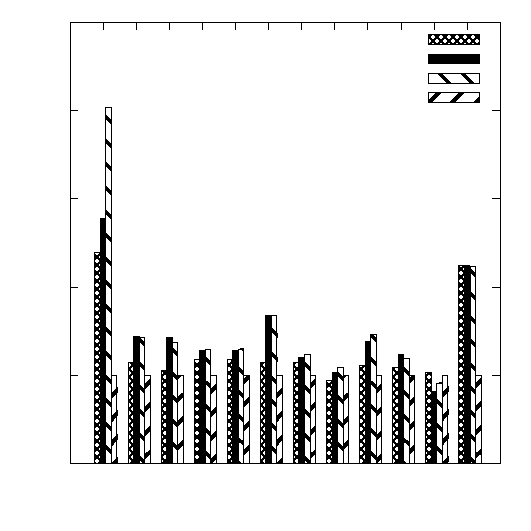
\includegraphics{spec}}%
    \gplfronttext
  \end{picture}%
\endgroup

	\caption{Prefetcher speedup chart}
	\label{fig:prefetcher_speedup}
\end{figure}

\subsection{Table Parameters}
We tested with different values for table size, pattern size and bits per address.
Fig.~\ref{fig:table_size_chart} shows the speedup with different table sizes.
Fig.~\ref{fig:pattern_size} shows the speedup with different pattern sizes.
Fig.~\ref{fig:bits} shows the results from using various bits per access.

\begin{figure}
	% GNUPLOT: LaTeX picture with Postscript
\begingroup
  \makeatletter
  \providecommand\color[2][]{%
    \GenericError{(gnuplot) \space\space\space\@spaces}{%
      Package color not loaded in conjunction with
      terminal option `colourtext'%
    }{See the gnuplot documentation for explanation.%
    }{Either use 'blacktext' in gnuplot or load the package
      color.sty in LaTeX.}%
    \renewcommand\color[2][]{}%
  }%
  \providecommand\includegraphics[2][]{%
    \GenericError{(gnuplot) \space\space\space\@spaces}{%
      Package graphicx or graphics not loaded%
    }{See the gnuplot documentation for explanation.%
    }{The gnuplot epslatex terminal needs graphicx.sty or graphics.sty.}%
    \renewcommand\includegraphics[2][]{}%
  }%
  \providecommand\rotatebox[2]{#2}%
  \@ifundefined{ifGPcolor}{%
    \newif\ifGPcolor
    \GPcolortrue
  }{}%
  \@ifundefined{ifGPblacktext}{%
    \newif\ifGPblacktext
    \GPblacktexttrue
  }{}%
  % define a \g@addto@macro without @ in the name:
  \let\gplgaddtomacro\g@addto@macro
  % define empty templates for all commands taking text:
  \gdef\gplbacktext{}%
  \gdef\gplfronttext{}%
  \makeatother
  \ifGPblacktext
    % no textcolor at all
    \def\colorrgb#1{}%
    \def\colorgray#1{}%
  \else
    % gray or color?
    \ifGPcolor
      \def\colorrgb#1{\color[rgb]{#1}}%
      \def\colorgray#1{\color[gray]{#1}}%
      \expandafter\def\csname LTw\endcsname{\color{white}}%
      \expandafter\def\csname LTb\endcsname{\color{black}}%
      \expandafter\def\csname LTa\endcsname{\color{black}}%
      \expandafter\def\csname LT0\endcsname{\color[rgb]{1,0,0}}%
      \expandafter\def\csname LT1\endcsname{\color[rgb]{0,1,0}}%
      \expandafter\def\csname LT2\endcsname{\color[rgb]{0,0,1}}%
      \expandafter\def\csname LT3\endcsname{\color[rgb]{1,0,1}}%
      \expandafter\def\csname LT4\endcsname{\color[rgb]{0,1,1}}%
      \expandafter\def\csname LT5\endcsname{\color[rgb]{1,1,0}}%
      \expandafter\def\csname LT6\endcsname{\color[rgb]{0,0,0}}%
      \expandafter\def\csname LT7\endcsname{\color[rgb]{1,0.3,0}}%
      \expandafter\def\csname LT8\endcsname{\color[rgb]{0.5,0.5,0.5}}%
    \else
      % gray
      \def\colorrgb#1{\color{black}}%
      \def\colorgray#1{\color[gray]{#1}}%
      \expandafter\def\csname LTw\endcsname{\color{white}}%
      \expandafter\def\csname LTb\endcsname{\color{black}}%
      \expandafter\def\csname LTa\endcsname{\color{black}}%
      \expandafter\def\csname LT0\endcsname{\color{black}}%
      \expandafter\def\csname LT1\endcsname{\color{black}}%
      \expandafter\def\csname LT2\endcsname{\color{black}}%
      \expandafter\def\csname LT3\endcsname{\color{black}}%
      \expandafter\def\csname LT4\endcsname{\color{black}}%
      \expandafter\def\csname LT5\endcsname{\color{black}}%
      \expandafter\def\csname LT6\endcsname{\color{black}}%
      \expandafter\def\csname LT7\endcsname{\color{black}}%
      \expandafter\def\csname LT8\endcsname{\color{black}}%
    \fi
  \fi
  \setlength{\unitlength}{0.0500bp}%
  \begin{picture}(5100.00,5100.00)%
    \gplgaddtomacro\gplbacktext{%
      \csname LTb\endcsname%
      \put(663,372){\makebox(0,0)[r]{\strut{} 1.03}}%
      \put(663,937){\makebox(0,0)[r]{\strut{} 1.04}}%
      \put(663,1503){\makebox(0,0)[r]{\strut{} 1.05}}%
      \put(663,2068){\makebox(0,0)[r]{\strut{} 1.06}}%
      \put(663,2634){\makebox(0,0)[r]{\strut{} 1.07}}%
      \put(663,3199){\makebox(0,0)[r]{\strut{} 1.08}}%
      \put(663,3764){\makebox(0,0)[r]{\strut{} 1.09}}%
      \put(663,4330){\makebox(0,0)[r]{\strut{} 1.1}}%
      \put(663,4895){\makebox(0,0)[r]{\strut{} 1.11}}%
      \put(765,186){\makebox(0,0){\strut{} 16}}%
      \put(1213,186){\makebox(0,0){\strut{} 32}}%
      \put(1660,186){\makebox(0,0){\strut{} 64}}%
      \put(2108,186){\makebox(0,0){\strut{} 128}}%
      \put(2555,186){\makebox(0,0){\strut{} 256}}%
      \put(3003,186){\makebox(0,0){\strut{} 512}}%
      \put(3450,186){\makebox(0,0){\strut{} 1024}}%
      \put(3898,186){\makebox(0,0){\strut{} 2048}}%
      \put(4345,186){\makebox(0,0){\strut{} 4096}}%
      \put(4793,186){\makebox(0,0){\strut{} 8192}}%
    }%
    \gplgaddtomacro\gplfronttext{%
    }%
    \gplbacktext
    \put(0,0){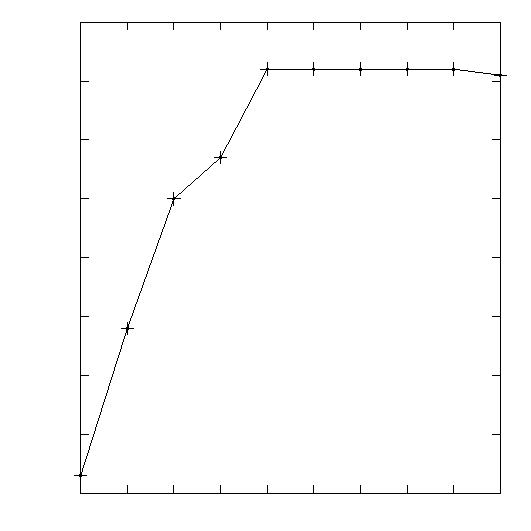
\includegraphics{tablesize}}%
    \gplfronttext
  \end{picture}%
\endgroup

	\caption{Speedup vs. table size}
	\label{fig:table_size_chart}
\end{figure}

\begin{figure}
	% GNUPLOT: LaTeX picture with Postscript
\begingroup
  \makeatletter
  \providecommand\color[2][]{%
    \GenericError{(gnuplot) \space\space\space\@spaces}{%
      Package color not loaded in conjunction with
      terminal option `colourtext'%
    }{See the gnuplot documentation for explanation.%
    }{Either use 'blacktext' in gnuplot or load the package
      color.sty in LaTeX.}%
    \renewcommand\color[2][]{}%
  }%
  \providecommand\includegraphics[2][]{%
    \GenericError{(gnuplot) \space\space\space\@spaces}{%
      Package graphicx or graphics not loaded%
    }{See the gnuplot documentation for explanation.%
    }{The gnuplot epslatex terminal needs graphicx.sty or graphics.sty.}%
    \renewcommand\includegraphics[2][]{}%
  }%
  \providecommand\rotatebox[2]{#2}%
  \@ifundefined{ifGPcolor}{%
    \newif\ifGPcolor
    \GPcolortrue
  }{}%
  \@ifundefined{ifGPblacktext}{%
    \newif\ifGPblacktext
    \GPblacktexttrue
  }{}%
  % define a \g@addto@macro without @ in the name:
  \let\gplgaddtomacro\g@addto@macro
  % define empty templates for all commands taking text:
  \gdef\gplbacktext{}%
  \gdef\gplfronttext{}%
  \makeatother
  \ifGPblacktext
    % no textcolor at all
    \def\colorrgb#1{}%
    \def\colorgray#1{}%
  \else
    % gray or color?
    \ifGPcolor
      \def\colorrgb#1{\color[rgb]{#1}}%
      \def\colorgray#1{\color[gray]{#1}}%
      \expandafter\def\csname LTw\endcsname{\color{white}}%
      \expandafter\def\csname LTb\endcsname{\color{black}}%
      \expandafter\def\csname LTa\endcsname{\color{black}}%
      \expandafter\def\csname LT0\endcsname{\color[rgb]{1,0,0}}%
      \expandafter\def\csname LT1\endcsname{\color[rgb]{0,1,0}}%
      \expandafter\def\csname LT2\endcsname{\color[rgb]{0,0,1}}%
      \expandafter\def\csname LT3\endcsname{\color[rgb]{1,0,1}}%
      \expandafter\def\csname LT4\endcsname{\color[rgb]{0,1,1}}%
      \expandafter\def\csname LT5\endcsname{\color[rgb]{1,1,0}}%
      \expandafter\def\csname LT6\endcsname{\color[rgb]{0,0,0}}%
      \expandafter\def\csname LT7\endcsname{\color[rgb]{1,0.3,0}}%
      \expandafter\def\csname LT8\endcsname{\color[rgb]{0.5,0.5,0.5}}%
    \else
      % gray
      \def\colorrgb#1{\color{black}}%
      \def\colorgray#1{\color[gray]{#1}}%
      \expandafter\def\csname LTw\endcsname{\color{white}}%
      \expandafter\def\csname LTb\endcsname{\color{black}}%
      \expandafter\def\csname LTa\endcsname{\color{black}}%
      \expandafter\def\csname LT0\endcsname{\color{black}}%
      \expandafter\def\csname LT1\endcsname{\color{black}}%
      \expandafter\def\csname LT2\endcsname{\color{black}}%
      \expandafter\def\csname LT3\endcsname{\color{black}}%
      \expandafter\def\csname LT4\endcsname{\color{black}}%
      \expandafter\def\csname LT5\endcsname{\color{black}}%
      \expandafter\def\csname LT6\endcsname{\color{black}}%
      \expandafter\def\csname LT7\endcsname{\color{black}}%
      \expandafter\def\csname LT8\endcsname{\color{black}}%
    \fi
  \fi
  \setlength{\unitlength}{0.0500bp}%
  \begin{picture}(5100.00,5100.00)%
    \gplgaddtomacro\gplbacktext{%
      \csname LTb\endcsname%
      \put(663,372){\makebox(0,0)[r]{\strut{} 1.05}}%
      \put(663,1126){\makebox(0,0)[r]{\strut{} 1.06}}%
      \put(663,1880){\makebox(0,0)[r]{\strut{} 1.07}}%
      \put(663,2634){\makebox(0,0)[r]{\strut{} 1.08}}%
      \put(663,3387){\makebox(0,0)[r]{\strut{} 1.09}}%
      \put(663,4141){\makebox(0,0)[r]{\strut{} 1.1}}%
      \put(663,4895){\makebox(0,0)[r]{\strut{} 1.11}}%
      \put(765,186){\makebox(0,0){\strut{} 1}}%
      \put(1213,186){\makebox(0,0){\strut{} 2}}%
      \put(1660,186){\makebox(0,0){\strut{} 3}}%
      \put(2108,186){\makebox(0,0){\strut{} 4}}%
      \put(2555,186){\makebox(0,0){\strut{} 5}}%
      \put(3003,186){\makebox(0,0){\strut{} 6}}%
      \put(3450,186){\makebox(0,0){\strut{} 7}}%
      \put(3898,186){\makebox(0,0){\strut{} 8}}%
      \put(4345,186){\makebox(0,0){\strut{} 9}}%
      \put(4793,186){\makebox(0,0){\strut{} 10}}%
    }%
    \gplgaddtomacro\gplfronttext{%
    }%
    \gplbacktext
    \put(0,0){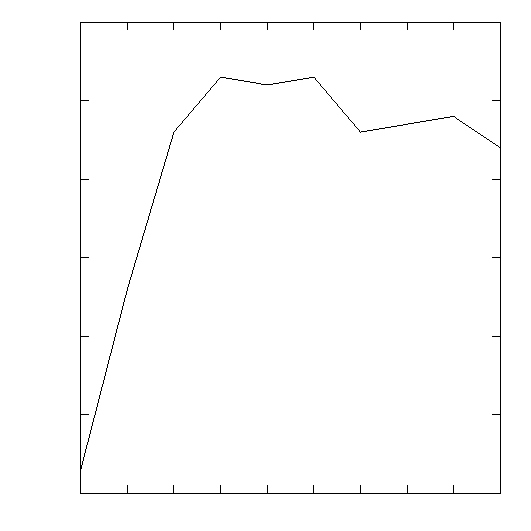
\includegraphics{patternsize}}%
    \gplfronttext
  \end{picture}%
\endgroup

	\caption{Speedup vs. pattern size}
	\label{fig:pattern_size}
\end{figure}

\begin{figure}
	% GNUPLOT: LaTeX picture with Postscript
\begingroup
  \makeatletter
  \providecommand\color[2][]{%
    \GenericError{(gnuplot) \space\space\space\@spaces}{%
      Package color not loaded in conjunction with
      terminal option `colourtext'%
    }{See the gnuplot documentation for explanation.%
    }{Either use 'blacktext' in gnuplot or load the package
      color.sty in LaTeX.}%
    \renewcommand\color[2][]{}%
  }%
  \providecommand\includegraphics[2][]{%
    \GenericError{(gnuplot) \space\space\space\@spaces}{%
      Package graphicx or graphics not loaded%
    }{See the gnuplot documentation for explanation.%
    }{The gnuplot epslatex terminal needs graphicx.sty or graphics.sty.}%
    \renewcommand\includegraphics[2][]{}%
  }%
  \providecommand\rotatebox[2]{#2}%
  \@ifundefined{ifGPcolor}{%
    \newif\ifGPcolor
    \GPcolortrue
  }{}%
  \@ifundefined{ifGPblacktext}{%
    \newif\ifGPblacktext
    \GPblacktexttrue
  }{}%
  % define a \g@addto@macro without @ in the name:
  \let\gplgaddtomacro\g@addto@macro
  % define empty templates for all commands taking text:
  \gdef\gplbacktext{}%
  \gdef\gplfronttext{}%
  \makeatother
  \ifGPblacktext
    % no textcolor at all
    \def\colorrgb#1{}%
    \def\colorgray#1{}%
  \else
    % gray or color?
    \ifGPcolor
      \def\colorrgb#1{\color[rgb]{#1}}%
      \def\colorgray#1{\color[gray]{#1}}%
      \expandafter\def\csname LTw\endcsname{\color{white}}%
      \expandafter\def\csname LTb\endcsname{\color{black}}%
      \expandafter\def\csname LTa\endcsname{\color{black}}%
      \expandafter\def\csname LT0\endcsname{\color[rgb]{1,0,0}}%
      \expandafter\def\csname LT1\endcsname{\color[rgb]{0,1,0}}%
      \expandafter\def\csname LT2\endcsname{\color[rgb]{0,0,1}}%
      \expandafter\def\csname LT3\endcsname{\color[rgb]{1,0,1}}%
      \expandafter\def\csname LT4\endcsname{\color[rgb]{0,1,1}}%
      \expandafter\def\csname LT5\endcsname{\color[rgb]{1,1,0}}%
      \expandafter\def\csname LT6\endcsname{\color[rgb]{0,0,0}}%
      \expandafter\def\csname LT7\endcsname{\color[rgb]{1,0.3,0}}%
      \expandafter\def\csname LT8\endcsname{\color[rgb]{0.5,0.5,0.5}}%
    \else
      % gray
      \def\colorrgb#1{\color{black}}%
      \def\colorgray#1{\color[gray]{#1}}%
      \expandafter\def\csname LTw\endcsname{\color{white}}%
      \expandafter\def\csname LTb\endcsname{\color{black}}%
      \expandafter\def\csname LTa\endcsname{\color{black}}%
      \expandafter\def\csname LT0\endcsname{\color{black}}%
      \expandafter\def\csname LT1\endcsname{\color{black}}%
      \expandafter\def\csname LT2\endcsname{\color{black}}%
      \expandafter\def\csname LT3\endcsname{\color{black}}%
      \expandafter\def\csname LT4\endcsname{\color{black}}%
      \expandafter\def\csname LT5\endcsname{\color{black}}%
      \expandafter\def\csname LT6\endcsname{\color{black}}%
      \expandafter\def\csname LT7\endcsname{\color{black}}%
      \expandafter\def\csname LT8\endcsname{\color{black}}%
    \fi
  \fi
  \setlength{\unitlength}{0.0500bp}%
  \begin{picture}(5100.00,5100.00)%
    \gplgaddtomacro\gplbacktext{%
      \csname LTb\endcsname%
      \put(663,372){\makebox(0,0)[r]{\strut{} 0.94}}%
      \put(663,875){\makebox(0,0)[r]{\strut{} 0.96}}%
      \put(663,1377){\makebox(0,0)[r]{\strut{} 0.98}}%
      \put(663,1880){\makebox(0,0)[r]{\strut{} 1}}%
      \put(663,2382){\makebox(0,0)[r]{\strut{} 1.02}}%
      \put(663,2885){\makebox(0,0)[r]{\strut{} 1.04}}%
      \put(663,3387){\makebox(0,0)[r]{\strut{} 1.06}}%
      \put(663,3890){\makebox(0,0)[r]{\strut{} 1.08}}%
      \put(663,4392){\makebox(0,0)[r]{\strut{} 1.1}}%
      \put(663,4895){\makebox(0,0)[r]{\strut{} 1.12}}%
      \put(765,186){\makebox(0,0){\strut{} 2}}%
      \put(1213,186){\makebox(0,0){\strut{} 4}}%
      \put(1660,186){\makebox(0,0){\strut{} 6}}%
      \put(2108,186){\makebox(0,0){\strut{} 8}}%
      \put(2555,186){\makebox(0,0){\strut{} 10}}%
      \put(3003,186){\makebox(0,0){\strut{} 12}}%
      \put(3450,186){\makebox(0,0){\strut{} 14}}%
      \put(3898,186){\makebox(0,0){\strut{} 16}}%
      \put(4345,186){\makebox(0,0){\strut{} 18}}%
      \put(4793,186){\makebox(0,0){\strut{} 20}}%
    }%
    \gplgaddtomacro\gplfronttext{%
    }%
    \gplbacktext
    \put(0,0){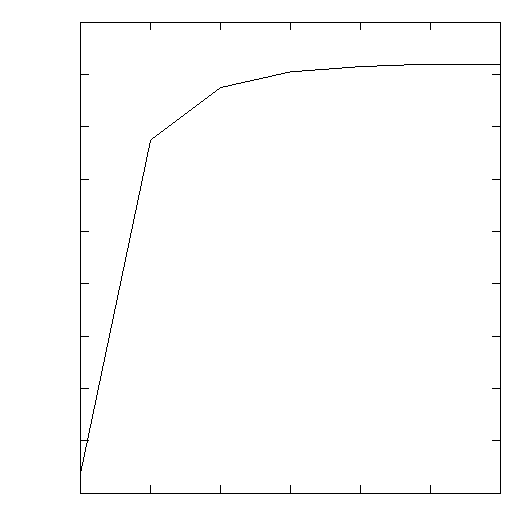
\includegraphics{bits}}%
    \gplfronttext
  \end{picture}%
\endgroup

	\caption{Speedup vs. bits per access}
	\label{fig:bits}
\end{figure}

\subsection{Pattern Matching Results}
For the pattern matching code we tried varying both aggressiveness and
threshold. Fig.~\ref{fig:aggr} shows the speedup with the aggressiveness set to
a fraction of the pattern size. We get the best result when the aggressiveness
is $\frac{5}{6}$ of the pattern size.

We also tried tuning the threshold, from perfect matching to various kinds of
partial matching, but the results were discouraging. Perfect matching was
better in all cases.

\begin{figure}
	% GNUPLOT: LaTeX picture with Postscript
\begingroup
  \makeatletter
  \providecommand\color[2][]{%
    \GenericError{(gnuplot) \space\space\space\@spaces}{%
      Package color not loaded in conjunction with
      terminal option `colourtext'%
    }{See the gnuplot documentation for explanation.%
    }{Either use 'blacktext' in gnuplot or load the package
      color.sty in LaTeX.}%
    \renewcommand\color[2][]{}%
  }%
  \providecommand\includegraphics[2][]{%
    \GenericError{(gnuplot) \space\space\space\@spaces}{%
      Package graphicx or graphics not loaded%
    }{See the gnuplot documentation for explanation.%
    }{The gnuplot epslatex terminal needs graphicx.sty or graphics.sty.}%
    \renewcommand\includegraphics[2][]{}%
  }%
  \providecommand\rotatebox[2]{#2}%
  \@ifundefined{ifGPcolor}{%
    \newif\ifGPcolor
    \GPcolortrue
  }{}%
  \@ifundefined{ifGPblacktext}{%
    \newif\ifGPblacktext
    \GPblacktexttrue
  }{}%
  % define a \g@addto@macro without @ in the name:
  \let\gplgaddtomacro\g@addto@macro
  % define empty templates for all commands taking text:
  \gdef\gplbacktext{}%
  \gdef\gplfronttext{}%
  \makeatother
  \ifGPblacktext
    % no textcolor at all
    \def\colorrgb#1{}%
    \def\colorgray#1{}%
  \else
    % gray or color?
    \ifGPcolor
      \def\colorrgb#1{\color[rgb]{#1}}%
      \def\colorgray#1{\color[gray]{#1}}%
      \expandafter\def\csname LTw\endcsname{\color{white}}%
      \expandafter\def\csname LTb\endcsname{\color{black}}%
      \expandafter\def\csname LTa\endcsname{\color{black}}%
      \expandafter\def\csname LT0\endcsname{\color[rgb]{1,0,0}}%
      \expandafter\def\csname LT1\endcsname{\color[rgb]{0,1,0}}%
      \expandafter\def\csname LT2\endcsname{\color[rgb]{0,0,1}}%
      \expandafter\def\csname LT3\endcsname{\color[rgb]{1,0,1}}%
      \expandafter\def\csname LT4\endcsname{\color[rgb]{0,1,1}}%
      \expandafter\def\csname LT5\endcsname{\color[rgb]{1,1,0}}%
      \expandafter\def\csname LT6\endcsname{\color[rgb]{0,0,0}}%
      \expandafter\def\csname LT7\endcsname{\color[rgb]{1,0.3,0}}%
      \expandafter\def\csname LT8\endcsname{\color[rgb]{0.5,0.5,0.5}}%
    \else
      % gray
      \def\colorrgb#1{\color{black}}%
      \def\colorgray#1{\color[gray]{#1}}%
      \expandafter\def\csname LTw\endcsname{\color{white}}%
      \expandafter\def\csname LTb\endcsname{\color{black}}%
      \expandafter\def\csname LTa\endcsname{\color{black}}%
      \expandafter\def\csname LT0\endcsname{\color{black}}%
      \expandafter\def\csname LT1\endcsname{\color{black}}%
      \expandafter\def\csname LT2\endcsname{\color{black}}%
      \expandafter\def\csname LT3\endcsname{\color{black}}%
      \expandafter\def\csname LT4\endcsname{\color{black}}%
      \expandafter\def\csname LT5\endcsname{\color{black}}%
      \expandafter\def\csname LT6\endcsname{\color{black}}%
      \expandafter\def\csname LT7\endcsname{\color{black}}%
      \expandafter\def\csname LT8\endcsname{\color{black}}%
    \fi
  \fi
  \setlength{\unitlength}{0.0500bp}%
  \begin{picture}(5100.00,5100.00)%
    \gplgaddtomacro\gplbacktext{%
      \csname LTb\endcsname%
      \put(765,372){\makebox(0,0)[r]{\strut{} 1.094}}%
      \put(765,1277){\makebox(0,0)[r]{\strut{} 1.096}}%
      \put(765,2181){\makebox(0,0)[r]{\strut{} 1.098}}%
      \put(765,3086){\makebox(0,0)[r]{\strut{} 1.1}}%
      \put(765,3990){\makebox(0,0)[r]{\strut{} 1.102}}%
      \put(765,4895){\makebox(0,0)[r]{\strut{} 1.104}}%
      \put(867,186){\makebox(0,0){\strut{}$\frac{1}{2}$}}%
      \put(1652,186){\makebox(0,0){\strut{}$\frac{2}{3}$}}%
      \put(2437,186){\makebox(0,0){\strut{}$\frac{3}{4}$}}%
      \put(3223,186){\makebox(0,0){\strut{}$\frac{4}{5}$}}%
      \put(4008,186){\makebox(0,0){\strut{}$\frac{5}{6}$}}%
      \put(4793,186){\makebox(0,0){\strut{}$1$}}%
    }%
    \gplgaddtomacro\gplfronttext{%
    }%
    \gplbacktext
    \put(0,0){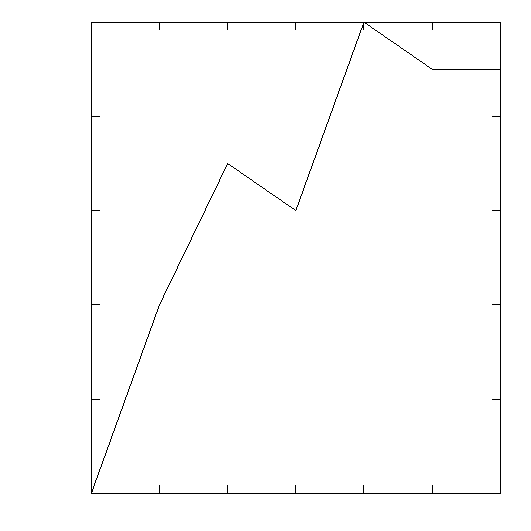
\includegraphics{aggr}}%
    \gplfronttext
  \end{picture}%
\endgroup

	\caption{Speedup vs. stride aggressiveness}
	\label{fig:aggr}
\end{figure}

\subsection{Most Common Stride Parameters}

For the most common stride part of the algorithm we tested different parameters
for aggressiveness and threshold. Fig.~\ref{fig:mcs_tweaks} shows the results
of the different simulations.
The reason for the extra data point for Threshold=4 was that the line went
up from 7 to 8. We therefore chose to run an extra test to check if the
trend continued with aggressiveness=9.

\begin{figure}
	% GNUPLOT: LaTeX picture with Postscript
\begingroup
  \makeatletter
  \providecommand\color[2][]{%
    \GenericError{(gnuplot) \space\space\space\@spaces}{%
      Package color not loaded in conjunction with
      terminal option `colourtext'%
    }{See the gnuplot documentation for explanation.%
    }{Either use 'blacktext' in gnuplot or load the package
      color.sty in LaTeX.}%
    \renewcommand\color[2][]{}%
  }%
  \providecommand\includegraphics[2][]{%
    \GenericError{(gnuplot) \space\space\space\@spaces}{%
      Package graphicx or graphics not loaded%
    }{See the gnuplot documentation for explanation.%
    }{The gnuplot epslatex terminal needs graphicx.sty or graphics.sty.}%
    \renewcommand\includegraphics[2][]{}%
  }%
  \providecommand\rotatebox[2]{#2}%
  \@ifundefined{ifGPcolor}{%
    \newif\ifGPcolor
    \GPcolortrue
  }{}%
  \@ifundefined{ifGPblacktext}{%
    \newif\ifGPblacktext
    \GPblacktexttrue
  }{}%
  % define a \g@addto@macro without @ in the name:
  \let\gplgaddtomacro\g@addto@macro
  % define empty templates for all commands taking text:
  \gdef\gplbacktext{}%
  \gdef\gplfronttext{}%
  \makeatother
  \ifGPblacktext
    % no textcolor at all
    \def\colorrgb#1{}%
    \def\colorgray#1{}%
  \else
    % gray or color?
    \ifGPcolor
      \def\colorrgb#1{\color[rgb]{#1}}%
      \def\colorgray#1{\color[gray]{#1}}%
      \expandafter\def\csname LTw\endcsname{\color{white}}%
      \expandafter\def\csname LTb\endcsname{\color{black}}%
      \expandafter\def\csname LTa\endcsname{\color{black}}%
      \expandafter\def\csname LT0\endcsname{\color[rgb]{1,0,0}}%
      \expandafter\def\csname LT1\endcsname{\color[rgb]{0,1,0}}%
      \expandafter\def\csname LT2\endcsname{\color[rgb]{0,0,1}}%
      \expandafter\def\csname LT3\endcsname{\color[rgb]{1,0,1}}%
      \expandafter\def\csname LT4\endcsname{\color[rgb]{0,1,1}}%
      \expandafter\def\csname LT5\endcsname{\color[rgb]{1,1,0}}%
      \expandafter\def\csname LT6\endcsname{\color[rgb]{0,0,0}}%
      \expandafter\def\csname LT7\endcsname{\color[rgb]{1,0.3,0}}%
      \expandafter\def\csname LT8\endcsname{\color[rgb]{0.5,0.5,0.5}}%
    \else
      % gray
      \def\colorrgb#1{\color{black}}%
      \def\colorgray#1{\color[gray]{#1}}%
      \expandafter\def\csname LTw\endcsname{\color{white}}%
      \expandafter\def\csname LTb\endcsname{\color{black}}%
      \expandafter\def\csname LTa\endcsname{\color{black}}%
      \expandafter\def\csname LT0\endcsname{\color{black}}%
      \expandafter\def\csname LT1\endcsname{\color{black}}%
      \expandafter\def\csname LT2\endcsname{\color{black}}%
      \expandafter\def\csname LT3\endcsname{\color{black}}%
      \expandafter\def\csname LT4\endcsname{\color{black}}%
      \expandafter\def\csname LT5\endcsname{\color{black}}%
      \expandafter\def\csname LT6\endcsname{\color{black}}%
      \expandafter\def\csname LT7\endcsname{\color{black}}%
      \expandafter\def\csname LT8\endcsname{\color{black}}%
    \fi
  \fi
  \setlength{\unitlength}{0.0500bp}%
  \begin{picture}(5100.00,5100.00)%
    \gplgaddtomacro\gplbacktext{%
      \csname LTb\endcsname%
      \put(951,595){\makebox(0,0)[r]{\strut{} 1.088}}%
      \put(951,1168){\makebox(0,0)[r]{\strut{} 1.09}}%
      \put(951,1742){\makebox(0,0)[r]{\strut{} 1.092}}%
      \put(951,2315){\makebox(0,0)[r]{\strut{} 1.094}}%
      \put(951,2888){\makebox(0,0)[r]{\strut{} 1.096}}%
      \put(951,3462){\makebox(0,0)[r]{\strut{} 1.098}}%
      \put(951,4035){\makebox(0,0)[r]{\strut{} 1.1}}%
      \put(951,4608){\makebox(0,0)[r]{\strut{} 1.102}}%
      \put(1053,409){\makebox(0,0){\strut{} 4}}%
      \put(1988,409){\makebox(0,0){\strut{} 5}}%
      \put(2923,409){\makebox(0,0){\strut{} 6}}%
      \put(3858,409){\makebox(0,0){\strut{} 7}}%
      \put(4793,409){\makebox(0,0){\strut{} 8}}%
      \put(144,2745){\rotatebox{-270}{\makebox(0,0){\strut{}Average speedup}}}%
      \put(2923,130){\makebox(0,0){\strut{}count}}%
    }%
    \gplgaddtomacro\gplfronttext{%
      \csname LTb\endcsname%
      \put(4005,4728){\makebox(0,0)[r]{\strut{}1}}%
      \csname LTb\endcsname%
      \put(4005,4542){\makebox(0,0)[r]{\strut{}2}}%
      \csname LTb\endcsname%
      \put(4005,4356){\makebox(0,0)[r]{\strut{}3}}%
      \csname LTb\endcsname%
      \put(4005,4170){\makebox(0,0)[r]{\strut{}4}}%
      \csname LTb\endcsname%
      \put(4005,3984){\makebox(0,0)[r]{\strut{}5}}%
    }%
    \gplbacktext
    \put(0,0){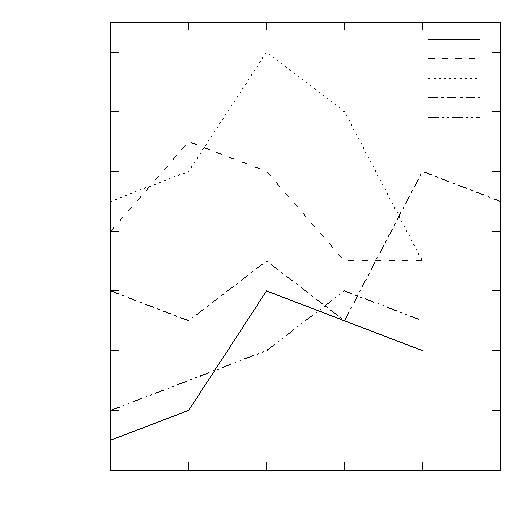
\includegraphics{mcs}}%
    \gplfronttext
  \end{picture}%
\endgroup

	\caption{Most Common Stride Threshold and Aggressiveness}
	\label{fig:mcs_tweaks}
\end{figure}


\section{Discussion}
The prefetcher presented in this report ...

\subsection{Table Parameters}
At a certain point the effect of giving the prefetcher more memory is virtually
zero. Fig.~\ref{fig:table_size_chart} shows that there seems to be no point in
having more than 256 entries. This we believe is caused by instruction
conflicts in the table. When the table reaches a certain size, most
instructions get their own place in the table, and avoid being evicted by
conflicting instructions.
A interesting observation is that it dips down at 8192 entries. This seems
to be due to a single benchmark, \emph{twolf}.

Fig.~\ref{fig:bits} shows the speedup related to bits per access.
We see a great increase up to 12 bits, then it slowly flattens out,
and we get the same speedup for 18 and 20 bits.
This is expected, as more bits allows bigger stride patterns to fit.

The last table parameter we changed was the maximum pattern size.
This was done by changing the number of accesses per entry.
With $2n+1$ accesses we can match patterns up to size $n$.
These results can be seen in Fig.~\ref{fig:pattern_size}.
We also see that there is not much gain in having more than 13
accesses per entry (13 accesses gives us a max pattern size of 6).
However when we tested adding more accesses per entry, and thus
increasing the maximum pattern size, we had the aggressiveness
set to the pattern size. Therefore it is possible that the bigger
patterns lead to a too high aggressiveness. It would be interesting
to run the tests with static aggressiveness to see if we saw the
same fall in performance above 13 accesses
per entry.

If we take the best of all these parameters we end up with a table size
of 256, 13 accesses per entry and 18 bits per access. This makes
the total table $256 \cdot 13 \cdot 18 = 59904 \textrm{ bits} = 7488 \textrm{ bytes}$ large.

\subsection{Other parameters}
An interesting result is shown in Fig.~\ref{fig:mcs_tweaks}.
We see that most common stride works best when the aggressiveness
is as high as six, and the threshold is at three.

It was also interesting to see that partial matching did not fare very well.
With this in mind one could optimize the algorithm by using relative strides
instead of absolute strides and only do perfect matching.


\section{Conclusion}
In this paper we have presented our own prefetcher based on the principles of strides. It tries to match patterns in the access history on a local (per PC) basis. We try to find a perfect match, and if this is not found, then we fall back on Most Common Stride.

After thorough tweaking of parameters, our prefetcher acheived a speedup of 1.102 compared to no prefetcher. 

\subsection{Future Work}

Prefetch alle most common stride

Aggressiveness most common stride avhengig av count

\todo{TODO: prefetch alle most common strides}


\bibliographystyle{IEEEtran}
\bibliography{bibliography}

\end{document}
